\documentclass[conference]{IEEEtran}
\IEEEoverridecommandlockouts

\usepackage{cite}
\usepackage{amsmath,amssymb,amsfonts}
\usepackage{algorithmic}
\usepackage{graphicx}
\usepackage{textcomp}
\usepackage{xcolor}
\usepackage{subfigure}
\usepackage[brazil]{babel}



\begin{document}



\title{Trabalho Intermediário de EEE928 -\\Extração de Caracteríticas}

\author{
\IEEEauthorblockN{Rafael Fernandes Gonçalves da Silva}
\IEEEauthorblockA{\textit{Departamento de Engenharia Elétrica} \\
\textit{Universidade Federal de Minas Gerais}\\
Belo Horizonte, Brasil \\
rafaelfgs@ufmg.br}
}

\maketitle

\begin{abstract}
O trabalho consiste em propor novas formas de realizar a extração de características em bases de dados de imagens. As características foram obtidas através da camada totalmente conectada de uma Rede Neural Convolucional (\textit{CNN}) . Para treinamento da rede, foi utilizado o método \textit{backpropagation} utilizando o erro gerado entre os valores de características obtidos e os valores determinados como ideais. Como base de dados, foram utilizados a \textit{MNIST} e a \textit{CIFAR10}, onde foram obtidos valores de acurácia satisfatórios.
\end{abstract}

\global\long\def\IEEEkeywordsname{Palavras-chave}
\begin{IEEEkeywords}
Rede Neural Convolucional, Extração de Características, \textit{backpropagation}, Máquinas de Vetores Suporte
\end{IEEEkeywords}



\section{Introdução} \label{intro}

As redes neurais convolucionais também, conhecidas como \textit{CNN's} (\textit{Convolutional Neural Networks}), são amplamente utilzadas como formas de resoluções de diversos problemas computacionais. Dentre eles pode-se citar o reconhecimento de expressões faciais, como realizado em \cite{cnnfacial}. Em \cite{cnnbio}, utilizou-se redes convolucionais para classificar textos biomédicos, mais especificamente em artigos de pesquisa e documentos clínicos. Pode também serem utilizadas em treinamentos não supervisionados, como descrito em \cite{cnnzeroshot}. \textit{CNN's} são aplicadas em \cite{cnngenome} para aprender atividades funcionais de sequências de DNA. Em \cite{cnnspeech}, utilizou-se dessas redes para tarefas de reconhecimento de fala contínua de grande vocabulário (\textit{LVCSR}). As redes neurais convolucionais também podem ser projetadas para segmentar imagens de tecidos cerebrais, conforme realizado em \cite{cnnbrain}.

A extração de características pode representar um método interessante quando visto de forma computacional. Através da extração, conforme explicado em \cite{ftguyon}, pode-se reduzir a quantidade de dados, aumentar o entendimento sobre a configuração dos dados, melhorar o desempenho da classificação e outras coisas mais. A extração de características do presente artigo consiste em retirar informações da camada totalmente conectada de uma rede e utilizá-las para o treinamento dessa rede.

Vários são os métodos para treinamento de redes neurais convolucionais. O \textit{backpropagation} representa um dos métodos mais antigos de treinamento, já sendo utilizado há algumas décadas, que consiste em propagar, de forma reversa na rede, derivadas para seus parâmetros. Porém, de acordo com \cite{bplecun}, esse método é ainda popular devido sua simplicidade conceitual e computacional, geralmente funcionando para vários tipos de base de entrada. Além disso, conforme \cite{bpzhang}, a derivação passo-a-passo dos parâmetros é de facil entendimento, ajudando os iniciantes no assunto.

Dentre os métodos de classificação, Máquinas de Vetores Suporte (\textit{SVM's}) são amplamente utilizadas atualmente. De acordo com \cite{svmwang}, podem ser usadas de forma linear ou não linear, através de transformadas dos dados de entrada, utilizando margens de separação entre as classes. Esse método possui um desempenho significativo, sendo utilizado na mais diversas áreas. Em \cite{svmfinanc}, \cite{svmchem}  e \cite{svmhydro} pode-se observar aplicações nas respectivas áreas financeira, química e hidrológica.

A base de dados utilizada em um treinamento corresponde outro assunto que possui uma grande variedade de perfis. As bases \textit{MNIST} e \textit{CIFAR10} são duas das mais comumente utilizadas atualmente. A primeira é mais simples e apresenta imagens dos dígitos de 0 à 9 escritos à mão. Possui apenas uma camada de cor (em escala de cinza), tendo 60000 amostras de treino e 10000 amostras de teste. Alguns dos dados da base \textit{MNIST} estão representados na Figura \ref{figmnist}. A base de dados \textit{CIFAR10} é um pouco mais complexa, possui 50000 amostras de treino e 10000 amostras de teste. Esta apresenta imagens coloridas (camadas de cores RGB), com valores de classes entre 0 e 9 representando os respectivos objetos: \textit{airplane}, \textit{automobile}, \textit{bird}, \textit{cat}, \textit{deer}, \textit{dog}, \textit{frog}, \textit{horse}, \textit{ship} e \textit{truck}. Parte dos dados dessa base está representada na Figura \ref{figcifar}.

Nesse artigo, será apresentada a utilização de uma rede neural convolucional treinada pelo método \textit{backpropagation} com as bases de dados \textit{MNIST} e \textit{CIFAR10}. O erro calculado na saída para iniciar a propagação das derivadas dos parâmetros foi obtido através da camada totalmente conectada, não sendo necessário um classificador dos dados durante o treinamento. Após o treinamento, os dados de saída são classificados através de \textit{SVM's} e é realizada a predição dos dados de teste.

\begin{figure}[h]
\centering
\subfigure[]{
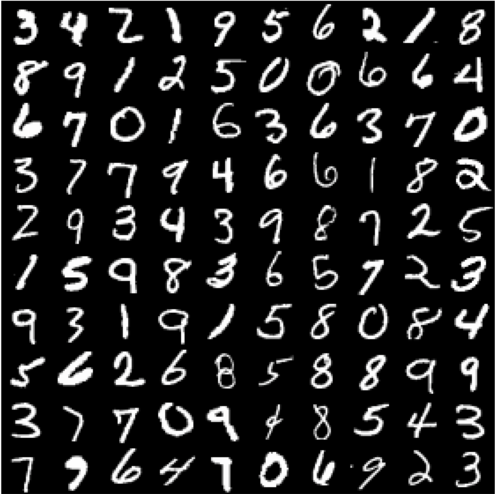
\includegraphics[width=.3\linewidth]{fig/mnist.png}
\label{figmnist}
}\quad
\subfigure[]{
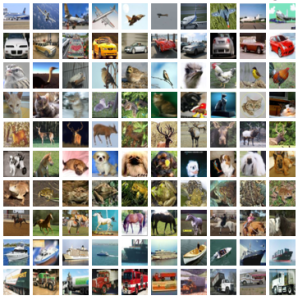
\includegraphics[width=.3\linewidth]{fig/cifar10.png}
\label{figcifar}
}
\caption{Parte da base de dados \textit{MNIST} (a) e \textit{CIFAR10} (b).}
\label{figbase}
\end{figure}


\section{Metodologia }\label{metod}

O objetivo desse trabalho consiste em dois treinamentos. O primeiro, de uma rede neural convolucional, utilizando a camada totalmente conectada para o cálculo do erro. O segundo é o treinamento do classificador, aplicado na rede já treinada, para realizar a predição das classes. Os passos utilizados nesse treinamento estão demonstrados nas subseções a seguir.

Foi proposto no trabalho a utilização da base de dados \textit{MNIST}. Os valores apresentados nessa seção correspondem àqueles obtidos para essa base. Os valores para outras bases estarão apresentados assim quando for necessário. Outra particularidade está na linguagem utilizada. Através do \textit{software} \textit{RStudio}, versão 1.2.1335, foi implementado um código na linguagem \textit{R}.



\subsection{Rede Neural Convolucional} \label{metod:struct}

A estrutura escolhida para a rede neural convolucional foi semelhante àquela apresentada por \cite{bpzhang}. Esta foi dividida em seis diferentes camadas e está representada na Figura \ref{figrede}. Inicialmente, uma rede é criada seguindo o padrão utilizado por \cite{bpzhang}. Os valores das máscaras utilizadas na convolução (representando os pesos da rede), são iniciados utilizando uma distribuição normal e dependentes do tamanho da máscara e da quantidade de camadas da entrada e da saída, conforme a equação \eqref{eqkernelrand}. Os limiares responsáveis pela ativação da rede são inicializados como nulos.

\begin{equation}
k_{p,q} = U \left ( \pm \sqrt { \frac {6} { ( inputsize + outputsize ) \times kernel^{2} } } \right  ) \label{eqkernelrand}
\end{equation}

\begin{figure}[b]
\centerline{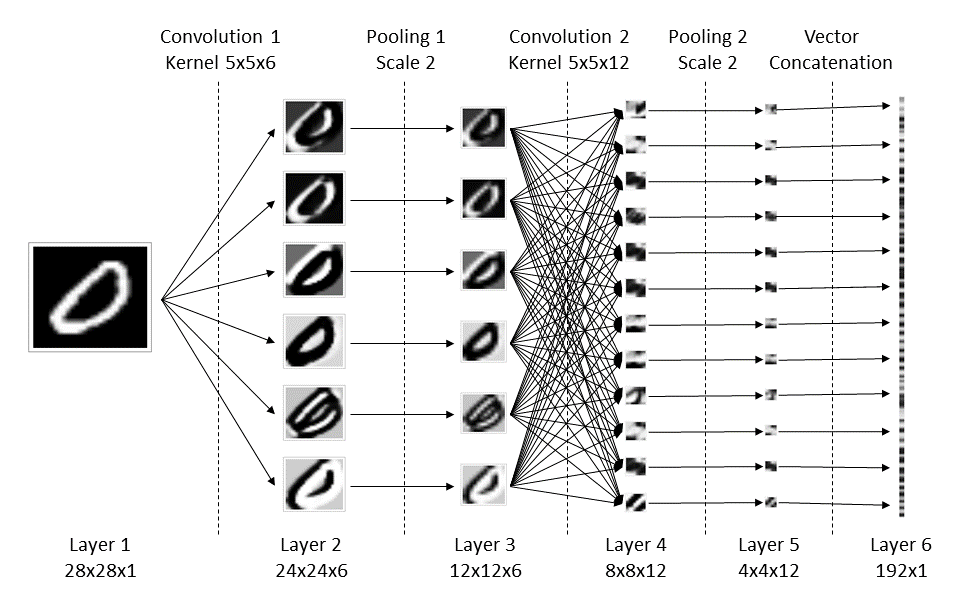
\includegraphics[width=.95\columnwidth]{fig/net.png}}
\caption{Estrutura da Rede Neural Convolucional utilizada aplicada em uma imagem da classe $0$ da base \textit{MNIST}.}
\label{figrede}
\end{figure}

A primeira camada da rede neural representa a entrada da rede. Nessa camada não é feita modificação alguma e sua saída é a própria imagem de entrada, com dimensão igual à 28x28x1.

A segunda camada representa uma camada de convolução. Neste ponto, passa-se seis máscaras de tamanho 5x5 com passo igual à 1 sobre a camada de saída anterior, representada pela imagem de entrada. Em seguida, a resposta é somada ao limiar e a ativação dessa camada ocorre de acordo com um sigmoide aplicado sobre o resultado dessa soma. Essa operação pode ser representada pelas equações \eqref{eqconv} e \eqref{eqsigm}:

\begin{equation}
z_{q} = \sum_{p=1}^{n} \left ( S_{p} \ast k_{p,q} \right ) + b_{q} \label{eqconv}
\end{equation}

\begin{equation}
\sigma = \frac {1} { 1 + e^{-z} } \label{eqsigm}
\end{equation}

onde $S_{p}$ é a \textit{p-ésima} camada da imagem de entrada, $n$ representa o número de camadas da imagem de entrada, $k_{p,q}$ é a máscara relacionada à \textit{p-ésima} camada da imagem de entrada e à \textit{q-ésima} camada da imagem de saída e $b_{q}$ é o limiar da \textit{q-ésima} camada da imagem de saída. De acordo com o tamanho e a quantidade das máscaras utilizado, a convolução irá produzir uma imagem de dimensão 24x24x6, representando a saída dessa camada.
 
A terceira camada representa um escalonamento de imagem, denominado \textit{pooling}. Este processo consiste em reduzir uma imagem através de um fator de escala. Neste trabalho, o tipo de escalonamento utilizado foi o \textit{average pooling}, com um fator de escala igual à 2, reduzindo pela metade o número de dados da imagem. A saída então será representada por um \textit{array} de dimensão 14x14x6. Pode-se notar que nesse método não é feito alterações na quantidade de camadas da imagem.

Na quarta camada há outra operação de convolução, ocorrendo de forma similar à da segunda camada, porém com doze diferentes máscaras. Foi criado um esquema para representar essa operação, mostrado na Figura \ref{figconv}. No esquema, é possivel observar algumas das camadas da imagem de entrada. Cada uma dessas camadas são convolucionadas com as doze máscaras, representadas por $k_{p,q}$, de acordo com \eqref{eqconv} e, após serem somadas aos doze diferentes limiares, representados por $b_{q}$, são ativados através de um sigmoide $\sigma$ calculado conforme \eqref{eqsigm}. A saída para essa camada será de dimensão 8x8x12.

\begin{figure}[b]
\centerline{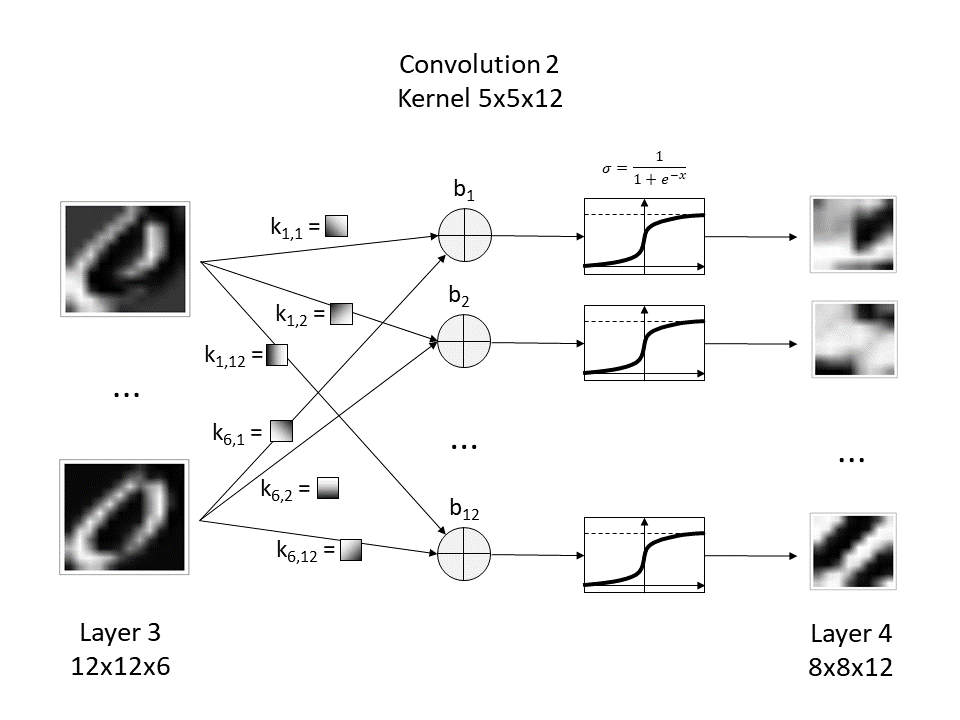
\includegraphics[width=.8\columnwidth]{fig/conv.png}}
\caption{Exemplo da segunda convolução realizada na quarta camada da rede para uma imagem da classe $0$ da base \textit{MNIST}.}
\label{figconv}
\end{figure}

A quinta camada é representada por um outro escalonamento de imagem com fator igual à 2, similar à terceira camada. Logo chega-se a valores de saída com dimensão igual à 4x4x12.

Por fim, na última camada é realizada uma transformação da saída da última camada em um vetor. Nesse ponto, foi utilizada a função $as.vector$, nativa da linguagem \textit{R}, a qual converte uma variável com parâmetros distribuídos em um vetor não distribuido. Como a ordem dos valores do vetor de saída mostrou-se irrelevante, a utilização dessa função mostrou-se eficiente, principalmente no seu tempo de execução. O tamanho do vetor de saída pode ser representado pelo produto das dimensões da entrada dessa camada, sendo igual à 128x1.



\subsection{Treinamento da rede} \label{metod:train}

Dada a rede neural convolucional criada, seu treinamento pode ser representado por um ciclo, que pode ser dividido em cinco partes, mostrado na Figura \ref{figcycle}. Para um melhor desempenho computacional, as imagens de entrada são divididas em pacotes de índices aleatórios que são lançados na rede. Cada entrada de um pacote de imagens representa uma iteração, onde os pesos e os limiares das camadas são atualizados.

A primeira refere-se ao \textit{feedfoward}, onde um pacote de imagens é definido como entrada. De acordo com os parâmetros atuais da rede, são determinadas de forma sequencial as saídas correspondentes à cada camada. As características utilizadas nos passos seguintes do ciclo são aquelas encontradas na sáida da última camada da rede.

\begin{figure}[b]
\centerline{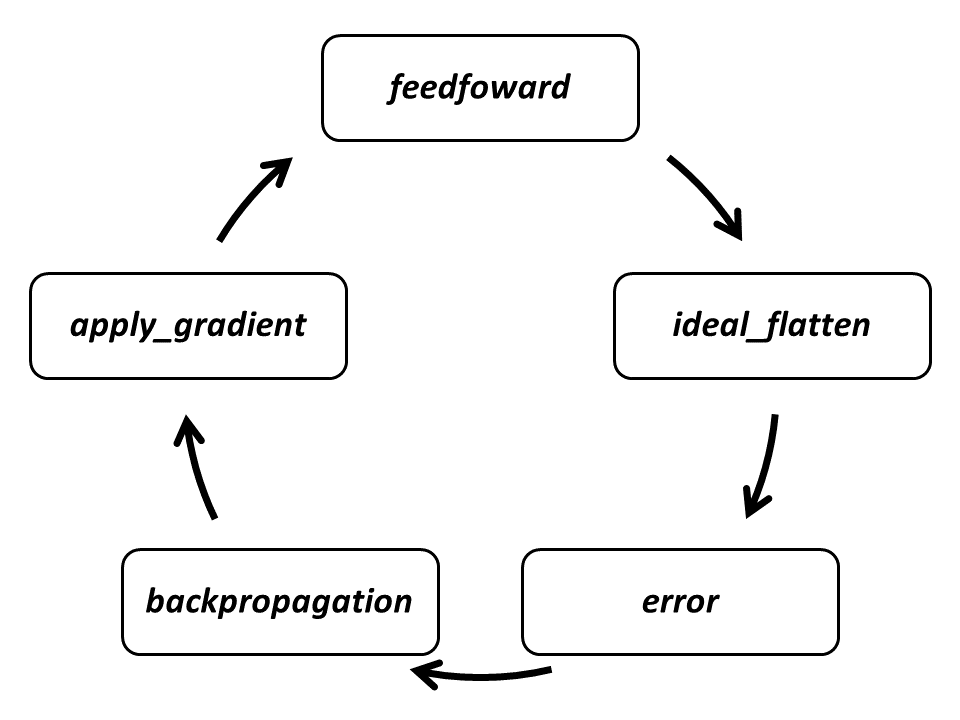
\includegraphics[width=.6\columnwidth]{fig/cycle.png}}
\caption{Ciclo utilizado no treinamento da rede.}
\label{figcycle}
\end{figure}

Na segunda parte do treinamento são obtidas as características ideais para as imagens de entrada. Para encontrar essa matriz, foi realizada uma sequência de passos. Primeiramente, utilizando a saída da última camada e os valores de suas respectivas classes, foi encontrada a média das características de cada classe. A Tabela \ref{tabmean} demonstra a média encontrada para dez características em um dado instante do treinamento. Em seguida, foi encontrada uma matriz que representa um histórico do andamento das classes, iniciada com valores nulos. A cada iteração, para uma característica qualquer, os valores encontrados na matriz anterior que estiverem abaixo da média são adicionados como -1 e caso estiverem abaixo da média são adicionados como 1 à essa matriz de histórico, mostrada na Tabela \ref{tabmem}. Utilizando essas duas matrizes, foi estabelecido que a segunda irá prevalecer caso, para uma característica qualquer, o histórico de alguma classe for maior que a média somada ao dobro do desvio padrão ou menor que a média subtraída do dobro do desvio padrão, resultando respectivamente em 1 ou 0 na matriz final. Para valores intermediários do histórico, a matriz final será dada pela matriz das médias, 1 para valores acima da média e 0, caso contrário. Por fim, é verificada a separação entre as colunas dessa matriz final, utilizando a média dos quadrados das diferenças entre elas, apresentada na Tabela \ref{taberr}. Caso algum desses valores for superior a 0.7 (valor determinado empiricamente, representando uma diferença de 30\% entre as classes), é realizada a separação entre as classes correspondentes à esse valor. A separação é determinada utilizando a matriz final e a matriz de médias da Tabela \ref{tabmean}, onde são trocados alguns dos valores semelhantes na matriz final entre as classes não separadas, observando a diferença entre eles na matriz de média (a quantidade de valores a serem trocados é proporcional à semelhança entre as classes encontrada na matriz da Tabela \ref{taberr}). Essa tentativa de separação é realizada quatro vezes, chagando-se a esse limite, ou ocorrendo algum erro no caminho, a tentativa de separação é finalizada e a matriz final continua com os valores atuais. Nesse ponto a matriz final é determinada como ideal para cada classe e utilizando os valores das classes do pacote atual, a matriz final é convertida para vetores de características ideais para a entrada dada.

Na terceira parte do treinamento, são gerados os erros através da diferença entre os vetores encontrados na iteração atual e o vetor ideal encontrado na parte anterior. Através desse erro é encontrado o valor de perda atual, correspondente à média das somas das colunas dos erros ao quadrado. Este cálculo está apresentado em \eqref{eqloss}, onde $i$ e $j$ representam as linhas e as colunas do erro $E$, $n$ é o número total de linhas de $E$ e a média é aplicada em um vetor de colunas. Com esse valor, pode-se ter uma noção da quantidade de características que não atingiram se valor ideal.

\begin{equation}
L = mean \left [ \sum_{i=1}^{n} E_{i,j}^{2} \right ] \label{eqloss}
\end{equation}

Na quarta parte do treinamento, através dos valores de erro encontrados na seção anterior, é utilizado o método \textit{backpropagation}, onde percorre-se a rede neural de trás pra frente e são determinadas as derivadas das saídas de cada camada, de forma a minimizar o erro. Em seguida, a rede é novamente percorrida, dessa vez no seu sentido normal, e são encontradas as derivadas dos pesos e dos limiares que correspondem aos valores das derivadas das saídas.

Na quinta e última parte do ciclo de treinamento, são aplicados os gradientes dos pesos de dos limiares. Para isso, seus valores atuais são somados aos valores de suas respectivas derivadas multiplicados pelo fator de treinamento determinado antes do treino. A partir daí, com os pesos e limiares atualizados, reinicia-se o ciclo aplicando novamente dados de entrada.

\begin{table}[h]
\caption{Média das dez primeiras características de cada classe para um dado instante do treinamento.}
\tabcolsep=0.18cm
\begin{center}
\begin{tabular}{ccccccccccc}
\hline
4 & 2 & 8 & 7 & 1 & 3 & 5 & 6 & 9 & 0 \\ \hline
0.66 & 0.27 & 0.65 & 0.71 & 0.25 & 0.29 & 0.67 & 0.37 & 0.84 & 0.76 \\
0.83 & 0.18 & 0.29 & 0.13 & 0.17 & 0.27 & 0.55 & 0.54 & 0.67 & 0.58 \\
0.37 & 0.76 & 0.37 & 0.15 & 0.15 & 0.13 & 0.27 & 0.77 & 0.15 & 0.76 \\
0.06 & 0.45 & 0.59 & 0.38 & 0.22 & 0.70 & 0.56 & 0.24 & 0.21 & 0.77 \\
0.82 & 0.27 & 0.78 & 0.72 & 0.37 & 0.45 & 0.87 & 0.69 & 0.94 & 0.76 \\
0.84 & 0.25 & 0.64 & 0.08 & 0.41 & 0.51 & 0.66 & 0.90 & 0.66 & 0.33 \\
0.34 & 0.83 & 0.67 & 0.15 & 0.59 & 0.21 & 0.39 & 0.91 & 0.13 & 0.52 \\
0.09 & 0.41 & 0.66 & 0.47 & 0.67 & 0.78 & 0.68 & 0.28 & 0.29 & 0.78 \\
0.81 & 0.24 & 0.68 & 0.74 & 0.75 & 0.53 & 0.70 & 0.60 & 0.84 & 0.62 \\
0.89 & 0.47 & 0.63 & 0.13 & 0.79 & 0.67 & 0.52 & 0.82 & 0.59 & 0.13 \\ \hline
\end{tabular}
\label{tabmean}
\end{center}
\end{table}

\begin{table}[h]
\caption{Histórico das dez primeiras características para um dado instante do treinamento.}
\tabcolsep=0.12cm
\begin{center}
\begin{tabular}{ccccccccccc}
\hline
4 & 2 & 8 & 7 & 1 & 3 & 5 & 6 & 9 & 0 \\ \hline
4819 & -7201 & -6805 & 6025 & 7023 & 4969 & -5761 & 4237 & 6873 & -6827 \\
3491 & -7201 & -5459 & 7101 & 6745 & 5593 & 5127 & -4803 & -7037 & -5425 \\
-5367 & -7013 & -6265 & -1895 & -6091 & 7119 & 6735 & -3007 & -7031 & 7065 \\
6221 & -6503 & 6969 & -7203 & -7113 & 7049 & -6813 & 5483 & -5483 & 2507 \\
6521 & -7165 & -6781 & 5385 & 7063 & 5795 & 1493 & 6177 & 6301 & -7113 \\
5325 & -6907 & -169 & 7081 & 5913 & -6117 & 7081 & 4315 & -7175 & -5913 \\
-5345 & 5555 & -6951 & -5301 & -6949 & 3921 & 7093 & 5433 & -7023 & 7109 \\
5831 & 6111 & 6967 & -7193 & -7007 & 6857 & -7085 & 6939 & -3177 & -3545 \\
1243 & 6425 & -4499 & 2217 & 6357 & 247 & -2067 & 4205 & 6519 & -7095 \\
-3073 & 7099 & 6311 & 6907 & 3583 & -7183 & 6933 & 4547 & -7159 & -1195 \\ \hline
\end{tabular}
\label{tabmem}
\end{center}
\end{table}

\begin{table}[h]
\caption{Semelhança entre as classes observada antes da separação para um dado instante de treino.}
\tabcolsep=0.18cm
\begin{center}
\begin{tabular}{c|cccccccccc}
   & 4 & 2 & 8 & 7 & 1 & 2 & 5 & 6 & 9 & 0 \\ \hline
4 & 1.00 & 0.33 & 0.73 & 0.53 & 0.66 & 0.46 & 0.52 & 0.59 & 0.43 & 0.26 \\
2 & 0.33 & 1.00 & 0.33 & 0.53 & 0.47 & 0.45 & 0.46 & 0.18 & 0.59 & 0.52 \\
8 & 0.73 & 0.33 & 1.00 & 0.33 & 0.51 & 0.52 & 0.32 & 0.68 & 0.54 & 0.40 \\
7 & 0.53 & 0.53 & 0.33 & 1.00 & 0.70 & 0.22 & 0.71 & 0.41 & 0.40 & 0.41 \\
1 & 0.66 & 0.47 & 0.51 & 0.70 & 1.00 & 0.38 & 0.46 & 0.47 & 0.67 & 0.14 \\
3 & 0.46 & 0.45 & 0.52 & 0.22 & 0.38 & 1.00 & 0.33 & 0.46 & 0.56 & 0.58 \\
5 & 0.52 & 0.46 & 0.32 & 0.71 & 0.46 & 0.33 & 1.00 & 0.54 & 0.15 & 0.56 \\
6 & 0.59 & 0.18 & 0.68 & 0.41 & 0.47 & 0.46 & 0.54 & 1.00 & 0.38 & 0.54 \\
9 & 0.43 & 0.59 & 0.54 & 0.40 & 0.67 & 0.56 & 0.15 & 0.38 & 1.00 & 0.34 \\
0 & 0.26 & 0.52 & 0.40 & 0.41 & 0.14 & 0.58 & 0.56 & 0.54 & 0.34 & 1.00
\end{tabular}
\label{taberr}
\end{center}
\end{table}

\begin{table}[h]
\caption{Valores ideais para as características separáveis de cada classe para um dado instante de treino.}
\tabcolsep=0.28cm
\begin{center}
\begin{tabular}{ccccccccccc}
\hline
4 & 2 & 8 & 7 & 1 & 3 & 5 & 6 & 9 & 0 \\ \hline
1 & 0 & 0 & 1 & 1 & 1 & 0 & 1 & 1 & 0 \\
1 & 0 & 0 & 1 & 1 & 1 & 1 & 0 & 0 & 0 \\
0 & 0 & 0 & 0 & 0 & 1 & 1 & 1 & 0 & 1 \\
1 & 0 & 1 & 0 & 0 & 1 & 0 & 1 & 0 & 1 \\
1 & 0 & 0 & 1 & 1 & 1 & 1 & 1 & 1 & 0 \\
1 & 0 & 1 & 1 & 1 & 0 & 1 & 1 & 0 & 0 \\
0 & 1 & 0 & 0 & 0 & 1 & 1 & 1 & 0 & 1 \\
1 & 1 & 1 & 0 & 0 & 1 & 0 & 1 & 0 & 0 \\
1 & 1 & 0 & 1 & 1 & 0 & 0 & 1 & 1 & 0 \\
0 & 1 & 1 & 1 & 1 & 0 & 1 & 1 & 0 & 0 \\ \hline
\end{tabular}
\label{tabFINAL}
\end{center}
\end{table}



\subsection{Treinamento do classificador} \label{metod:svm}

Depois do treinamento da rede, foi realizado o treinamento do classificador através dos valores das características, representados pela saída da última camada da rede. Foi utilizado Máquinas de Vetores Suporte (\textit{SVM's}) como classificador das classes para as dadas características.

Utilizando parte do treinamanto da rede neural convolucional (\textit{feedfoward}), foram lançados na rede todos dados de treino da base \textit{MNIST}. Na última camada, a saída resultante foi uma matriz 192x60000, representando as 60000 características de cada entrada, associada a sua respectiva classe.

Através da função $svm$ do \textit{R}, presente na biblioteca $e1071$, utilizando a transposta da matriz das características e as respectivas classes, obteve-se um modelo do classificador das classes para a saída da rede neural convolucional.



\begin{table*}[h]
\caption{Valores preditos (colunas) para cada classe do \textit{MINST} (linhas).}
\begin{center}
\begin{tabular}{c|cccccccccc}
   & 0           & 1            & 2           & 3           & 4            & 5           & 6           & 7            & 8           & 9           \\ \hline
0 & 99.1\% &   0.0\% &   0.0\% &   0.0\% &   0.1\% &   0.2\% &   0.3\% &   0.1\% &   0.2\% &   0.0\% \\
1 &   0.0\% & 99.6\% &   0.2\% &   0.0\% &   0.0\% &   0.0\% &   0.1\% &   0.1\% &   0.0\% &   0.0\% \\
2 &   0.1\% &   0.0\% & 98.8\% &   0.3\% &   0.1\% &   0.0\% &   0.2\% &   0.4\% &   0.1\% &   0.0\% \\
3 &   0.0\% &   0.0\% &   0.3\% & 98.1\% &   0.0\% &   0.7\% &   0.0\% &   0.4\% &   0.5\% &   0.0\% \\
4 &   0.1\% &   0.0\% &   0.1\% &   0.0\% & 99.0\% &   0.0\% &   0.3\% &   0.0\% &   0.1\% &   0.4\% \\
5 &   0.3\% &   0.1\% &   0.0\% &   1.1\% &   0.0\% & 98.1\% &   0.1\% &   0.1\% &   0.0\% &   0.1\% \\
6 &   0.3\% &   0.2\% &   0.1\% &   0.0\% &   0.1\% &   0.4\% & 98.7\% &   0.0\% &   0.1\% &   0.0\% \\
7 &   0.0\% &   0.1\% &   1.0\% &   0.3\% &   0.1\% &   0.0\% &   0.0\% & 98.4\% &   0.0\% &   0.1\% \\
8 &   0.2\% &   0.2\% &   0.2\% &   0.6\% &   0.1\% &   0.4\% &   0.1\% &   0.1\% & 97.7\% &   0.3\% \\
9 &   0.1\% &   0.0\% &   0.0\% &   0.3\% &   0.3\% &   0.4\% &   0.0\% &   0.5\% &   0.2\% & 98.2\%
\end{tabular}
\label{tabemnist}
\end{center}
\end{table*}

\begin{table*}[h]
\caption{Valores preditos (colunas) para cada classe do \textit{CIFAR10} (linhas).}
\begin{center}
\begin{tabular}{c|cccccccccc}
                  & aiplane  & automobile & bird        & cat         & deer     & dog       & frog       & horse    & ship       & truck     \\ \hline
aiplane       & 56.0\% &        4.5\% &   4.0\% &   3.0\% &   3.2\% &   2.1\% &   1.9\% &   4.4\% & 14.8\% &   6.1\% \\
automobile &   3.7\% &      58.0\% &   2.0\% &   2.4\% &   0.9\% &   1.7\% &   1.5\% &   2.7\% & 11.1\% & 16.0\% \\
bird            &   6.9\% &        2.5\% & 27.3\% & 10.3\% & 18.2\% &   8.5\% & 12.4\% &   8.6\% &   2.8\% &   2.5\% \\
cat             &   3.5\% &        2.2\% &   7.6\% & 31.2\% &   7.7\% & 15.3\% & 17.6\% &   7.8\% &   3.6\% &   3.5\% \\
deer           &   4.8\% &        1.6\% &   6.7\% &   8.8\% & 39.9\% &   6.8\% & 15.2\% & 10.6\% &   3.0\% &   2.6\% \\
dog             &   2.1\% &        2.5\% &   9.3\% & 18.9\% & 10.0\% & 31.3\% & 11.8\% &   9.2\% &   3.1\% &   1.8\% \\
frog            &   0.7\% &        1.5\% &   5.5\% &   9.3\% & 12.0\% &   6.3\% & 58.2\% &   3.7\% &   0.9\% &   1.9\% \\
horse          &   5.5\% &        2.4\% &   4.3\% &   6.2\% &   9.5\% &   8.4\% &   5.1\% & 52.9\% &   1.9\% &   3.8\% \\
ship             & 19.3\% &        7.9\% &   1.5\% &   4.2\% &   0.8\% &   1.9\% &   1.5\% &   2.0\% & 52.8\% &   8.1\% \\
truck           &   6.8\% &      17.2\% &   1.8\% &   3.1\% &   1.5\% &   1.7\% &   3.0\% &   5.7\% & 11.8\% & 47.4\%
\end{tabular}
\label{tabecifar}
\end{center}
\end{table*}



\section{Resultados e Discussão} \label{Result}

Para o treinamento da rede, foram definidos padrões para alguns parâmetros: utilização de todos os dados de treino, uma taxa de aprendizagem de $0.2$ e pacotes com tamanho fixo de 50. Para o treinamento do classificador, foi utilizado um \textit{kernel} do tipo radial e um custo de violação de restrições igual à 10.

Os resultados desse trabalho foram obtidos em um Notebook Acer Aspire V3-571, utilizando o Windows 10 Home 64 bits, com um processador Intel® Core™ i7-3632QM CPU @ 2.20GHz, memória RAM 8,00GB 1333MHz e driver de vídeo Intel® HD Graphics 4000.

\subsection{Base de dados \textit{MNIST}} \label{result:mnist}

Para a base de dados \textit{MNIST}, foram utilizadas seis épocas de treinamento da rede, tendo uma duração de 3 horas e 4 minutos. Para pacotes de tamanho 50 e uma base de treino com 60000 imagens, o treino foi resultante de 7200 iterações. Os valores calculados de perda, através de \eqref{eqloss}, para cada iteração estão apresentados na Figura \ref{figlmnist}.

Pode-se observar que princípio do treinamento está ocorrendo como esperado, visto que a função de perda diminui a cada iteração. O ruído encontrado no valores de perda ocorre devido ao tamanho reduzido dos pacotes. Aumentar essa quantidade provocaria um menor ruído, mas reduziria o número de iterações e, consequentemente, as aplicações do gradiente.

\begin{figure}[b]
\centerline{\includegraphics[width=.8\columnwidth]{fig/L_mnist.png}}
\caption{Valores de perda encontrados durante seis épocas de treinamento da base \textit{MNIST} com pacotes de tamanho 50.}
\label{figlmnist}
\end{figure}

Para o treinamento classificador \textit{SVM}, foram utilizados os 60000 dados de treino e foi executado com um tempo de 22 minutos e 53 segundos.

Para obter os resultados de acurácia, foram utilizados os 10000 dados de teste da base \textit{MNIST}. Esses dados foram lançados na rede e a saída encontrada na última camada representou, de forma transposta, os dados de entrada para a predição. Esta foi determinada através da função $predict$, nativa da linguagem \textit{R}, e como argumentos foram utilizados os dados citados anteriomente e o modelo encontrado no treinamento do classificador. Realizando a média dos acertos para essas previsões obteve-se um resultado de 98.57\%.

Foi também encontrada a acurácia entre as classes, utlizando o mesmo príncipio anteriormente apresentado. Os valores encontrados estão na Tabela \ref{tabemnist}. Através desse resultado, é possível observar algumas peculiaridades. Os números com maior dificuldade de acerto foram o 8 e o 5, com taxas de acerto respectivas à 97.7\% e 98.1\%. As trocas mais comuns foram a classificação do 5 como 3 e do 7 como 2, com valores superiores à 1\%. O melhor resultado observado foi para a classe 1, com 99.6\% de acerto.



\subsection{Base de dados \textit{CIFAR10}} \label{result:cifar}

Para demonstrar a funcionalidade do código implementado, foi utilizada a base de dados \textit{CIFAR10} para treinamento da rede neural convolucional, não havendo alteração alguma no código. Para esta, foram utilizadas quatro épocas de treinamento da rede, tendo uma duração de 3 horas e 57 minutos. Neste caso, o treino foi resultante de 4000 iterações. Os valores calculados de perda para cada iteração estão apresentados na Figura \ref{figlcifar}.

Os 8GB de memória \textit{RAM} do \textit{hardware} disponível não foram suficientes para realizar o treinamento classificador \textit{SVM} com os 50000 dados de treino da base \textit{CIFAR10}, visto que o uso de imagens coloridas aumenta consideravelmente o uso de memória. Para isso, essa quantidade foi reduzida para 20000. Nesse caso, ainda foram observados picos de uso de memória próximos à 5.5GB, logo este pode ser considerado um fator limitante pelo \textit{hardware}. Utilizando então 20000 imagens obtidas de forma aleatória da base \textit{CIFAR10}, observou-se um tempo de treino igual à 19 minutos e 54 segundos.

\begin{figure}[h]
\centerline{\includegraphics[width=.8\columnwidth]{fig/L_cifar10.png}}
\caption{Valores de perda encontrados durante seis épocas de treinamento da base \textit{CIFAR10} com pacotes de tamanho 50.}
\label{figlcifar}
\end{figure}

De forma similar à base \textit{MNIST}, foram obtidos os resultados de acurácia através da função $predict$, utilizando as características encontradas na última camada da rede com os 10000 dados de teste da \textit{CIFAR10}. A média dos acertos apresentada para as previsões foi igual à 45.50\%.

Também foram encontrados os valores de acurácias entre as classes, cujos resultados estão na Tabela \ref{tabecifar}. Através dela, pode-se observar uma menor aproximação entre os valores preditos e os valores reais. A pior classificação ocorreu para a classe \textit{bird}, com 27.3\% de acerto, sendo esta confundida com várias outras. A pior confusão ocorreu na classe \textit{ship}, sendo confundida com a classe \textit{airplane} em 19.3\% dos casos. Os melhores resultados foram das classes \textit{frog} e \textit{automobile} com 58.2\% e 58.0\% de acerto.

Mesmo com altos valores de confusão, pode-se perceber que estes ocorreram entre classes mais próximas. As classes que representam animais obtiveram erros maiores quando comparadas entre si, mas erros menores quando comparadas com os meios de transporte. A mesma relação pode ser observada de forma contrária.


\section{Conclusão} \label{Concl}

Os resultados obtidos nesse trabalho apresentaram um desempenho satisfatório quando comparado a outros resultados de trabalhos similares.

Neste trabalho, o tempo demonstrou-se como um obstáculo para a execução do código, visto que cada época para a base de dados \textit{MNIST} era executada em cerca de 30 minutos e cada época da \textit{CIFAR10} em cerca de 1h. Um maior tempo de treinamento das redes ou a utilização de melhores \textit{hardwares} poderiam apresentar melhores resultados finais. De forma similar, uma maior disponibilidade de memória \textit{RAM} poderia melhorar o treinamento do classificado para a base \textit{CIFAR10}, conforme explicado na subseção \ref{result:cifar}

Durante a implementação do código, foram criadas três versões, cada uma com algum avanço em relação à outra. Na primeira, só havia a criação da matriz ideal de características baseada na média, sem garantir a separação, apresentando resultados de acurácia inferiores à 90\%. Na segunda versão, foi implementada a separação das colunas da matriz ideal de características, apresentando resultados próximos à 96\%. Nese ponto, foi observada uma alta variação nos valores da matriz ideal ao utilizar somente a média como base, logo, na versão atual, foi adicionado o histórico da matriz ideal deixando o treinamento da rede mais estável, visto que a matriz objetivo não apresentava valores com alta oscilação.

A principal proposta para futuros trabalhos é a implementação de uma forma de separação com algum embasamento teórico. A forma de separação atual baseia-se na matriz de médias das características das classes e realiza trocas de parte da matriz ideal das classes que não estão separadas, algo muito próximo à tentativa e erro. Esse método funcionou para as classes utilizadas, porém a utilização de métodos melhores formulados pode aumentar o desempenho final.

Outro fato importante nesse trabalho foi a utilização da média como forma de criar e serapar as colunas da matriz de características ideais. Este método também possui resultados satisfatórios para a base de dados \textit{MNIST} e \textit{CIFAR10}, podendo apresentar algumas limitações para bases com maior complexidade.

Por fim, de forma a aumentar o desempenho dos resultados, pode-se aplicar alguns dos métodos apresentados em \cite{ftguyon}: rejeitando ou aceitando características baseado nas suas respectivas relevâncias, ou levando em consideração a dependência entre as características.



\bibliographystyle{IEEEtran}
\bibliography{referencias} \label{Ref}



\end{document}